%% ──────────────────────────────────────────────────────────────────
%%  Diabetic Retinopathy — Lab 5 Report (v2)
%%  Computer Vision, April 2026
%% ──────────────────────────────────────────────────────────────────
\documentclass[a4paper, 10pt, twocolumn]{article}

\usepackage[top=1.8cm, bottom=1.8cm, left=1.4cm, right=1.4cm, columnsep=0.65cm]{geometry}
\usepackage[utf8]{inputenc}
\usepackage[T1]{fontenc}
\usepackage{lmodern}
\usepackage{microtype}
\usepackage{booktabs}
\usepackage{multirow}
\usepackage{pgfplots}
\pgfplotsset{compat=1.18}
\usepackage{xcolor}
\usepackage{titlesec}
\usepackage[hidelinks]{hyperref}
\usepackage{enumitem}
\usepackage{amsmath}
\usepackage[labelfont=bf, font=small, skip=3pt]{caption}
\usepackage{tabularx}
\usepackage{graphicx}

%% ── Colour palette ────────────────────────────────────────────────
\definecolor{accent}{RGB}{0, 64, 128}
\definecolor{rowbest}{RGB}{220, 240, 220}
\definecolor{rowbad} {RGB}{255, 230, 230}
\definecolor{rownorm}{RGB}{250, 250, 252}
\definecolor{rulecolor}{RGB}{0, 64, 128}

%% ── Section headings ─────────────────────────────────────────────
\titleformat{\section}
  {\normalfont\bfseries\small\color{accent}}
  {}{0em}{}[{\color{rulecolor}\vspace{-1pt}\hrule height 0.6pt\vspace{1pt}}]
\titlespacing{\section}{0pt}{5pt}{1pt}

\titleformat{\subsection}
  {\normalfont\small\bfseries}
  {}{0em}{}
\titlespacing{\subsection}{0pt}{2pt}{1pt}

%% ── Paragraph / list style ───────────────────────────────────────
\setlength{\parskip}{1pt}
\setlength{\parindent}{0pt}
\setlist[itemize]{topsep=0pt, itemsep=0pt, leftmargin=10pt,
                  label=\raisebox{0.3ex}{\tiny$\bullet$}, parsep=0pt}

%% ── Captions ─────────────────────────────────────────────────────
\setlength{\abovecaptionskip}{3pt}
\setlength{\belowcaptionskip}{0pt}

%% ══════════════════════════════════════════════════════════════════
\begin{document}

%% ── Title spanning both columns ──────────────────────────────────
\twocolumn[{%
\begin{center}
  {\large\bfseries\color{accent}
    Automatic Diagnosis of Diabetic Retinopathy\\[2pt]
    via Custom CNN Architecture and Transfer Learning}\\[4pt]
  {\small
    Maria Muñoz Pérez \enspace$\cdot$\enspace
    Cristina Sobrino Fernández-Miranda\enspace$\cdot$\enspace
    Computer Vision --- Lab 5 \enspace$\cdot$\enspace April 2026}\\[3pt]
  {\color{rulecolor}\hrule height 0.8pt}
  \vspace{5pt}
\end{center}
}]

%% ── 1. INTRODUCTION ──────────────────────────────────────────────
\section{Introduction}

Diabetic Retinopathy (DR) is a leading cause of preventable blindness.
We train a binary DR/No-DR classifier from fundus photographs under two
competition tracks: a \emph{custom} CNN trained from scratch (CUSTOM)
and a \emph{fine-tuned} pretrained backbone (FINE-TUNING).
Performance is measured by AUC on a held-out 1\,000-image test set
evaluated via Codabench.

%% ── 2. DATASET & PREPROCESSING ──────────────────────────────────
\section{Dataset \& Preprocessing}

The dataset contains 2\,000 training / 500 validation / 1\,000 test
fundus images with a class imbalance of 73\% No-DR / 27\% DR.
Right-eye images are horizontally mirrored to unify anatomical orientation.

\textbf{Shared preprocessing.}
\texttt{CropByEye} detects the retinal disc via intensity thresholding.
Ben Graham contrast normalisation~\cite{graham2015kaggle}
($4{\times}$orig $-$ $4{\times}$Gaussian-blur $+$ 128; sigmaX=10,
circular background mask) enhances microaneurysms and vessel edges.

\textbf{Custom pipeline (224\,px).}
Rescale to 256\,px; random horizontal flip, vertical flip,
rotation ($\pm$15°), colour jitter, random 224\,px crop (training);
centre crop (val/test). ImageNet normalisation.

\textbf{Fine-tuning pipeline (380\,px).}
Rescale to 416\,px; random horizontal flip, rotation ($\pm$180°),
colour jitter, random 380\,px crop (training); centre crop (val/test).
Rationale for the higher resolution and wider rotation is given in §\,4.

%% ── 3. CUSTOM MODEL ──────────────────────────────────────────────
\section{Custom Model (CUSTOM)}

\subsection{Architecture Evolution}

\textbf{CustomNet (baseline).}
4-block CNN with 5$\times$5 no-padding convolutions (3→6→16→32→64),
BatchNorm + MaxPool per block, flattened to 6\,400-d, head
6400→120→84→Dropout(0.5)→1. Optimiser: SGD + StepLR.
Result: 0.570 pub / 0.597 priv.

\textbf{CustomNetV2.}
Redesigned for better generalisation on a small dataset:
\begin{itemize}
  \item 5 blocks, 3$\times$3 same-padding convolutions
        (3→32→64→128→256→256), MaxPool per block.
  \item \textbf{Global Average Pooling} replaces the 6\,400-d flatten
        (256 scalars output), giving translation invariance.
  \item Head: Dropout(0.2)→Linear(256,128)→ReLU→
        Dropout(0.4)→Linear(128,1). $\approx$1\,M parameters.
  \item AdamW (lr=1e-3, wd=5e-3), CosineAnnealingLR($T_\text{max}$=50),
        50 epochs, patience=10.
\end{itemize}
Adding \texttt{WeightedRandomSampler} and BenGraham preprocessing
brings the public AUC to 0.770.

\subsection{Final Model: 3-Seed Ensemble}

Three independent runs of CustomNetV2 (seeds 42, 123, 456); outputs
averaged with 4-pass TTA per model. Diversity comes from random
weight initialisation and batch ordering — no architectural complexity
that could overfit on 2\,000 images.
Codabench: \textbf{0.757 pub / 0.780 priv} (best valid CUSTOM result).

\vspace{20pt}
%% ── 4. FINE-TUNING MODEL ─────────────────────────────────────────
\section{Fine-tuning Model (FINE-TUNING)}

\subsection{Backbone Selection}

\textbf{EfficientNet-B0} (baseline, SGD + StepLR): 0.698.
Switching to AdamW + CosineAnnealingLR and two-stage progressive
unfreezing raised this to 0.770, but persistent overfitting remained:
train AUC 0.957 vs.\ val 0.779 at best checkpoint (gap 0.178,
Fig.\,\ref{fig:curves}).\\


\textbf{DenseNet121}~\cite{huang2017densely} was chosen as a replacement.
Dense connections pass feature maps from all prior layers to every
subsequent layer within a block, acting as an implicit regulariser
and preventing any single layer from memorising the training set.
It is also the standard backbone for medical imaging benchmarks (CheXNet).
Head: Dropout(0.5)→Linear(1024,\,1). \\

\subsection{Two-Stage Progressive Unfreezing}
\textit{Stage\,1}:
\begin{itemize}
    \item  freeze entire backbone; unfreeze
    \item \texttt{denseblock4\,+\,norm5} ($\approx$2.16\,M trainable params).
    \item AdamW lr=3e-4, CosineAnnealingLR($T_\text{max}$=30), 30 epochs, patience=7.
\end{itemize}

\textit{Stage\,2}:
\begin{itemize}
    \item  additionally unfreeze \texttt{denseblock3\,+\,transition3}.
    \item Per-group LRs: backbone 3e-5, head 1e-4.
    \item Scheduler: 3-epoch linear warmup then CosineAnnealingLR($T_\text{max}$=12). The warmup prevents gradient spikes when newly unfrozen, unadapted layers  first receive the fine-tuning learning rate.
    \item Gate: Stage\,2 only runs if Stage\,1\,+\,TTA val AUC\,$\geq$\,0.752; reverts to Stage\,1 weights if AUC regresses.
\end{itemize}

\subsection{Multi-Backbone Ensemble}

Four backbones trained with the same two-stage strategy:
\textbf{DenseNet121}, \textbf{DenseNet169}, \textbf{ResNeXt50-32x4d},
and \textbf{SE-ResNeXt50-32x4d}.
Each captures complementary features: dense reuse (DenseNets),
grouped convolutions (ResNeXt), channel attention (SE-ResNeXt).
Val-set grid search over all 2/3/4-backbone combinations and discrete
weights selects the best blend. Single-model AUCs (TTA-4):
DenseNet121 0.780, DenseNet169 0.785, ResNeXt50 \textbf{0.806},
SE-ResNeXt50 0.778.
Best 4-backbone ensemble: Codabench \textbf{0.810}.

\subsection{Resolution \& Rotation Scaling (Final Model)}

\textbf{380\,px input.} Microaneurysms are the earliest DR lesion
(10--125\,$\mu$m diameter). At 224\,px they are $\approx$2\,px wide,
below the reliable detection threshold of a 3$\times$3 filter. At
380\,px they reach 3--4\,px. Abramoff et al.~\cite{abramoff2018pivotal}
identify resolution as the primary driver of sensitivity for early DR
lesion detection. All backbones use GlobalAveragePooling and require
no code change to handle 380\,px. Batch size reduced to 32/128 to fit GPU.

\textbf{$\pm$180° rotation.} Fundus cameras can be oriented at any angle;
there is no anatomically correct upright direction. The previous $\pm$15°
window discarded 92\% of valid rotations. Graham~\cite{graham2015kaggle}
identified full 360° rotation as the most important augmentation for
fundus DR detection.

\textbf{Final ensemble.} Grid search over all 2/3/4-backbone combinations
selects DenseNet121\,(0.35)\,+\,DenseNet169\,(0.15)\,+\,ResNeXt50\,(0.50).
SE-ResNeXt50 is excluded: it adds a weaker, correlated model that dilutes
the ensemble without contributing complementary diversity.
Val AUC: 0.8671. Codabench: \textbf{0.835 pub / 0.826 priv}.

%% ── 5. TRAINING SETUP ────────────────────────────────────────────
\section{Training Setup}

\textbf{Class-imbalance.}
\texttt{BCEWithLogitsLoss(pos\_weight\,$\approx$\,2.76)} addresses imbalance
at the gradient level. \texttt{WeightedRandomSampler} oversamples the
minority class at the batch level ($+$0.022 AUC). Both are used together.

\textbf{Test-Time Augmentation (TTA).}
4-pass: original, horizontal flip, vertical flip, 180° rotation.
Score is the mean of sigmoid outputs across all four passes
($+$0.008--0.012 AUC). Vertical flip is inference-only (not added to
training) to preserve the pretrained model's upright-prior distribution.

\textbf{Label Smoothing.}
For the fine-tuned backbone only ($\varepsilon$=0.05): hard $\{0,1\}$
targets become soft $\{0.025, 0.975\}$. Reduces overconfident logits
without harming the limited training signal~\cite{muller2019label}.


%% ── 6. ABLATIONS & NEGATIVE RESULTS ─────────────────────────────
\section{Ablations \& Negative Results}

\begin{itemize}
  \item \textbf{CLAHE preprocessing}: altered intensity distribution;
    broke \texttt{CropByEye}'s threshold ($-$4.6\% custom AUC).
    Permanently banned.
  \item \textbf{BenGraham uint8 bug}: \texttt{clip(uint8,0,1)} collapsed
    all pixels to $\{0,1\}$; the subtraction formula produced uniform grey 128.
    Both models trained on identical grey images (custom 0.541, FT 0.558).
    Fixed with a dtype guard and circular mask.
  \item \textbf{Pre-cached images}: a fixed 224\,px centre-crop at cache
    creation removed per-epoch \texttt{RandomCrop} jitter — the primary
    spatial regulariser on 2\,000 images ($-$0.028 AUC despite 5$\times$ speedup).
  \item \textbf{SE blocks on CustomNetV2}: channel attention overfits on
    2\,000 images; val AUC dropped $-$0.066 vs plain CustomNetV2.
  \item \textbf{Residual connections (CustomNetV3)}: marginal or no gain;
    skip connections add value only in very deep networks where vanishing
    gradients are a bottleneck.
  \item \textbf{DenseNet Stage\,3 unfreeze}: adding a third unfreezing stage
    (denseblock2\,+\,transition2) overfits (FT $-$0.013). Stages 1+2 are
    the optimal stopping point.
  \item \textbf{EfficientNet-B4-NS at 380\,px}: CUDA OOM (14.56\,GiB GPU,
    batch=16). Dropped; four smaller backbones retained.
  \item \textbf{rot90/rot270 in TTA (8-pass)}: BenGraham combined with
    rectangular crops breaks 90° rotational invariance. Rotated images
    fall outside the training distribution; AUC decreases for both models.
\end{itemize}

%% ══════════════════════════════════════════════════════════════════
%% PAGE 2 — TABLES, FIGURES & REFERENCES
%% ══════════════════════════════════════════════════════════════════
\newpage
\onecolumn

\section*{\color{accent}Supplementary Material: Tables, Figures and References}
{\color{rulecolor}\hrule height 0.6pt}
\vspace{4pt}

%% ── TABLE 1 (full width) ──────────────────────────────────────────
\captionof{table}{%
  AUC results for key submitted experiments
  (\emph{pub}\,=\,public leaderboard, \emph{priv}\,=\,private).
  \textbf{Bold}: best valid result per category.
  $^\dagger$\,Competition-invalid submission (reference only).
  \textit{Red rows}: failed experiments.}
\label{tab:results}
\vspace{3pt}
\footnotesize
\setlength{\tabcolsep}{4pt}
\renewcommand{\arraystretch}{1.10}
\begin{tabularx}{\textwidth}{@{}lXcc@{}}
\toprule
\textbf{Notebook} & \textbf{Key change} &
  \textbf{Custom AUC} & \textbf{FT AUC} \\
 & & \scriptsize pub\;/\;priv & \scriptsize pub\;/\;priv \\
\midrule
\texttt{first\_attempt}
  & EfficientNet-B0 (SGD) + CustomNet baseline
  & 0.570\;/\;0.597 & 0.698\;/\;0.708 \\
\texttt{attempt\_with\_c}
  & FT: AdamW + CosineAnnealingLR (SGD\,$\to$\,AdamW)
  & 0.561\;/\;0.579 & 0.751\;/\;0.734 \\
\texttt{second\_attempt\_tuned}
  & CustomNetV2 + WeightedRandomSampler + 2-stage FT + TTA-2
  & 0.766\;/\;0.743 & 0.770\;/\;0.744 \\
\rowcolor{rowbad}
\texttt{fourth\_attempt}
  & \textit{BenGraham uint8 bug — all images collapsed to grey}
  & \textit{0.541\;/\;0.557} & \textit{0.558\;/\;0.533} \\
\texttt{fifth\_attempt}
  & BenGraham fixed + 4-pass TTA + label smoothing
  & 0.770\;/\;0.770 & 0.757\;/\;0.755 \\
\rowcolor{rowbest}
\texttt{sixth\_attempt}$^\dagger$
  & DenseNet121 with 2-stage unfreezing + warmup scheduler
  & 0.786\;/\;0.787$^\dagger$ & 0.781\;/\;0.781$^\dagger$ \\
\texttt{seventh\_attempt}
  & DenseNet Stage\,3 unfreeze (overfits, reverted)
  & 0.756\;/\;0.762 & 0.768\;/\;0.754 \\
\texttt{attempt\_22} (eighth)
  & FT: ResNet50 (IMAGENET1K\_V2) replaces DenseNet121
  & 0.756\;/\;0.764 & 0.780\;/\;0.791 \\
\texttt{attempt\_21} (ninth)
  & FT: 4-backbone ensemble — DenseNet121/169, ResNeXt50, SE-ResNeXt50
  & 0.757\;/\;0.780 & 0.806\;/\;0.807 \\
\rowcolor{rowbest}
\texttt{attempt\_24} (tenth)
  & FT: 380\,px input + $\pm$180° rotation + 3-backbone weighted ensemble
  & 0.760\;/\;0.773 & \textbf{0.835\;/\;0.826} \\
\rowcolor{rowbest}
\texttt{ninth\_attempt}
  & Custom: plain CustomNetV2, 3-seed ensemble (seeds 42/123/456)
  & \textbf{0.757\;/\;0.780} & — \\
\bottomrule
\end{tabularx}

\vspace{10pt}

%% ── TABLE 2 + FIGURE (side by side) ──────────────────────────────
\begin{minipage}[t]{0.47\textwidth}

\captionof{table}{Architecture comparison: CustomNet vs CustomNetV2.}
\label{tab:arch}
\vspace{3pt}
\footnotesize
\setlength{\tabcolsep}{4pt}
\renewcommand{\arraystretch}{1.10}
\begin{tabular}{@{}lcc@{}}
\toprule
\textbf{Feature} & \textbf{CustomNet} & \textbf{CustomNetV2} \\
\midrule
Conv blocks  & 4 (5$\times$5, no-pad)    & 5 (3$\times$3, same-pad) \\
Channels     & 3→6→16→32→64              & 3→32→64→128→256→256 \\
Spatial head & Flatten (6\,400-d)        & Glob.\ Avg Pool (256-d) \\
FC head      & 6400→120→84→1            & 256→128→1 \\
Conv bias    & Yes                       & No (BN absorbs) \\
Optimiser    & SGD                       & AdamW (wd=5e-3) \\
LR schedule  & StepLR ($\gamma$=0.1)    & CosineAnnealingLR \\
Sampler      & Uniform                   & Weighted (class freq.) \\
Preprocessing& None                      & BenGraham \\
TTA          & None                      & 4-pass \\
\midrule
Seeds        & 1                         & 3 (ensemble) \\
Public AUC   & 0.570                     & \textbf{0.757} (valid) \\
\bottomrule
\end{tabular}

\end{minipage}%
\hfill
\begin{minipage}[t]{0.50\textwidth}

%% ── FIGURE 1 ─────────────────────────────────────────────────────
\captionof{figure}{EfficientNet-B0 Stage\,1 training curves
(\texttt{second\_attempt\_tuned}). Train AUC reaches 0.957 at the
best val checkpoint ($\star$, epoch\,14) while val AUC peaks at 0.779 —
a gap of 0.178. This motivated switching to DenseNet121, which
eliminated the gap (pub and priv AUC both 0.781).}
\label{fig:curves}
\vspace{3pt}

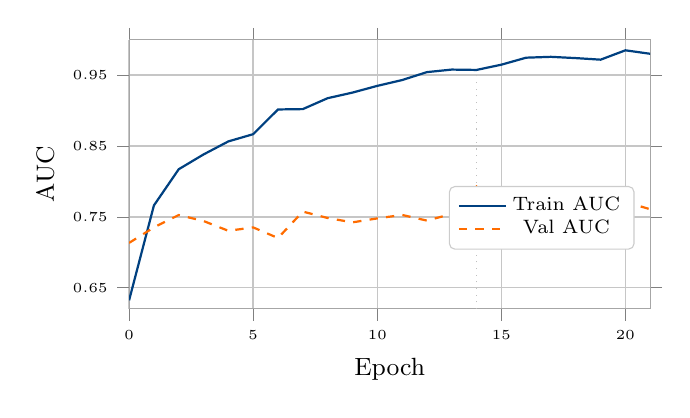
\begin{tikzpicture}
\begin{axis}[
  width  = 8.2cm,
  height = 5.0cm,
  xlabel = {Epoch},
  ylabel = {AUC},
  xmin=0, xmax=21,
  ymin=0.62, ymax=1.00,
  xtick={0,5,10,15,20},
  ytick={0.65,0.75,0.85,0.95},
  tick label style={font=\tiny},
  label style={font=\small},
  legend style={
    font=\scriptsize,
    at={(0.97,0.22)}, anchor=south east,
    draw=gray!40, fill=white, rounded corners=2pt,
    row sep=-2pt,
  },
  grid=both,
  grid style={line width=0.3pt, draw=gray!25},
  major grid style={line width=0.5pt, draw=gray!45},
  tick align=outside,
  axis line style={gray!70},
]

\addplot[color=accent, thick, mark=none] coordinates {
  (0,0.6322)(1,0.7661)(2,0.8172)(3,0.8381)(4,0.8565)
  (5,0.8667)(6,0.9016)(7,0.9021)(8,0.9175)(9,0.9254)
  (10,0.9349)(11,0.9431)(12,0.9543)(13,0.9579)(14,0.9574)
  (15,0.9648)(16,0.9747)(17,0.9759)(18,0.9741)(19,0.9719)
  (20,0.9851)(21,0.9802)
};
\addlegendentry{Train AUC}

\addplot[color=orange!85!red, thick, dashed, mark=none] coordinates {
  (0,0.7132)(1,0.7351)(2,0.7526)(3,0.7441)(4,0.7303)
  (5,0.7351)(6,0.7201)(7,0.7574)(8,0.7484)(9,0.7422)
  (10,0.7478)(11,0.7527)(12,0.7447)(13,0.7541)(14,0.7793)
  (15,0.7696)(16,0.7682)(17,0.7622)(18,0.7706)(19,0.7643)
  (20,0.7711)(21,0.7607)
};
\addlegendentry{Val AUC}

\addplot[only marks, mark=star, mark size=4pt, color=orange!85!red]
  coordinates { (14,0.7793) };
\addplot[gray!50, thin, dotted] coordinates { (14,0.62) (14,0.9574) };

\end{axis}
\end{tikzpicture}

\end{minipage}

\vspace{10pt}

%% ── REFERENCES ───────────────────────────────────────────────────
\renewcommand{\refname}{\normalfont\bfseries\small\color{accent}References}
\begin{thebibliography}{9}
\small\setlength{\itemsep}{1pt}

\bibitem{graham2015kaggle}
Graham, B. (2015).
Kaggle diabetic retinopathy detection competition report.
\textit{University of Warwick}.

\bibitem{huang2017densely}
Huang, G., Liu, Z., van der Maaten, L., \& Weinberger, K.\,Q. (2017).
Densely connected convolutional networks.
\textit{Proc.\ CVPR 2017}, 4700--4708.

\bibitem{abramoff2018pivotal}
Abramoff, M.\,D., et al. (2018).
Pivotal trial of an autonomous AI-based diagnostic system for detection of
diabetic retinopathy in primary care offices.
\textit{npj Digital Medicine}, 1(1), 39.

\bibitem{loshchilov2019adamw}
Loshchilov, I., \& Hutter, F. (2019).
Decoupled weight decay regularization.
\textit{Proc.\ ICLR 2019}.

\bibitem{muller2019label}
Müller, R., Kornblith, S., \& Hinton, G. (2019).
When does label smoothing help?
\textit{Proc.\ NeurIPS 2019}, 4694--4703.

\bibitem{tan2019efficientnet}
Tan, M., \& Le, Q.\,V. (2019).
EfficientNet: Rethinking model scaling for convolutional neural networks.
\textit{Proc.\ ICML 2019}.

\end{thebibliography}

\end{document}
